\section{Process}

In this section, we briefly review the architecture of the system for gathering and storing temperature sensor data, and then explain the setup of the parameter estimation problem using iterative proportional fitting.

\if 0
do we need this?
Approach: "quick" overview section
- explicitly what we're going to do
- how we're going to do it
- "now we go into more detail" etc

Architecture of System:
- sensors, database:
    - KETI and the Soda deployment
- data processing pipeline:
    - need for data cleaning; complications w/ sensors ('real world')
    - how to do data cleaning, the transformations we did
- Octave script to run IPF, generate edge parameters:
    - what would the results look like and what would we expect?

Problem Setup:
- how do decompose the space, the buildings, etc we used into graph
- go over options in how we could have represented:
    - bucketing temperature
    - more nodes; more accurate? more sensors
\fi

\begin{figure}[ht]
\centering
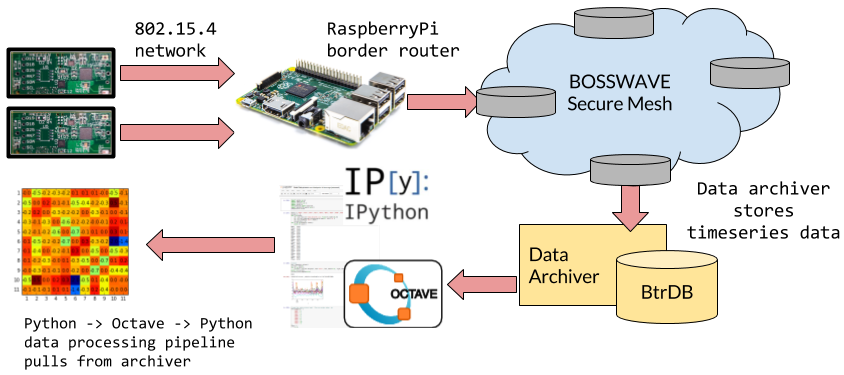
\includegraphics[width=.8\linewidth]{figs/281arch}
\caption{Overview of data acquisition and processing pipeline}
\label{fig:architecture}
\end{figure}


\subsection{Architecture}




\subsection{Problem Setup}
